\documentclass[11pt]{article}

%Don't change any thing before \begin{document}
%In fact if you use sth fancy, you might need
%to add more packages, or macros.
\usepackage{amssymb,amsmath}
\usepackage{amsthm}
\usepackage{times,psfrag,epsf,epsfig,graphics,graphicx}
\usepackage{algorithm}
\usepackage{algorithmic}


\title{CSCI 338: Assignment~2~(7 points)}
\author{River Kelly}
%\date{}
\date{Feb 18, 2021}


\begin{document}
\maketitle

%When writing up your solution, comment out the following until you reach Problem 1.
% \noindent
% This assignment is due on {\bf Thursday, Feb 18, 8:00pm}. It is strongly encouraged that you use Latex to generate a single pdf file and upload it under {\em Assignment 2} on D2L. But there will NOT be a penalty for not using Latex (to finish the assignment). This is {\bf not} a group-assignment, so you must finish the assignment by yourself.
\newpage
\section*{Problem 1}
% (1.1) Problem 1.6.d, 1.6.e (page 84--- all the questions with only numbers given are referred to the 3rd edition of the textbook, if not sure check with me during the face-to-face sessions).
\noindent
\textbf{1.1} Give state diagrams of DFAs recognizing the following languages. In all parts, the alphabet is $\{0,1\}$.
\newline
\newline
\textbf{1.6.d} 
\newline
$\{w \mid w \text{ has length at least 3 and its third symbol is a } 0\}$
\begin{center}
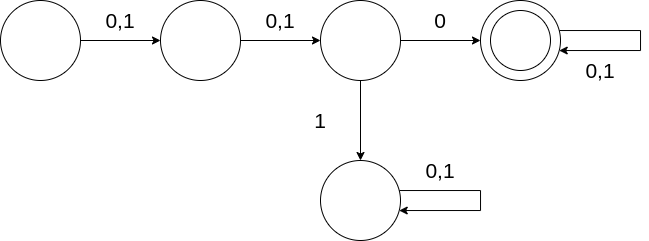
\includegraphics[scale=0.5]{02/HW02-1.6.d.png}    
\end{center}


\textbf{1.6.e} 
\newline
$ \{ w \mid w$ starts with $0$ and has odd length, or starts with 1 and has even length \}
\begin{center}
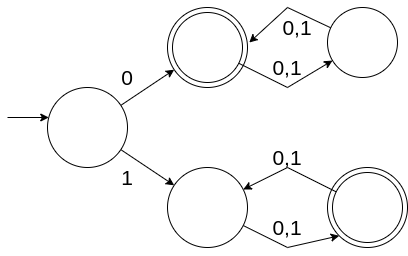
\includegraphics[scale=0.5]{02/HW02-1.6.e.png}    
\end{center}
\newpage
\noindent
\textbf{1.2} Give state diagrams of NFAs with the specified number of states recognizing each of the following languages. In all parts, the alphabet is $\{0,1\}$.
\newline
\newline
\textbf{1.7.b} 
The language of Exercise 1.6c with five states.
\newline
\newline
Five states that accept the strings over the alphabet $\Sigma=\{0,1\}$ and contains the sub-string 0101.
\begin{center}
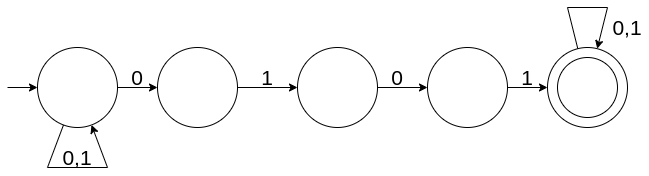
\includegraphics[scale=0.5]{02/HW02-1.7.b.png}    
\end{center}
\noindent
\textbf{1.7.c}
The language of Exercise 1.6l with six states
\begin{center}
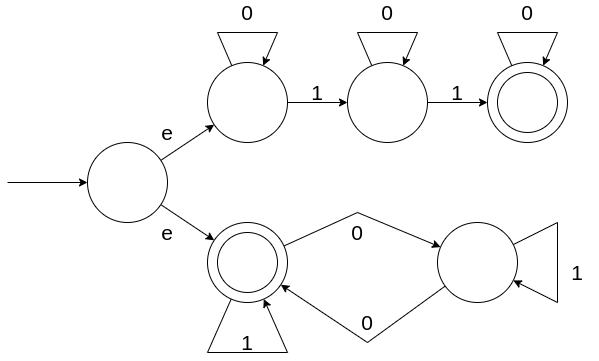
\includegraphics[scale=0.5]{02/HW02-1.7.c.png}    
\end{center}


\newpage
\section*{Problem 2}

Problem 1.16.a, ~Problem 1.16.b (page 86).

\textbf{1.16.a}
\begin{center}
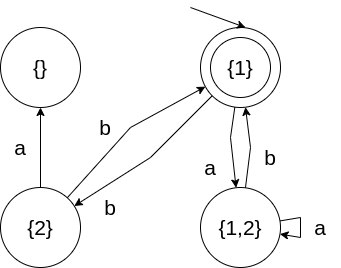
\includegraphics[scale=0.7]{02/HW02-1.16.a.png}    
\end{center}
\textbf{1.16.b}
\begin{center}
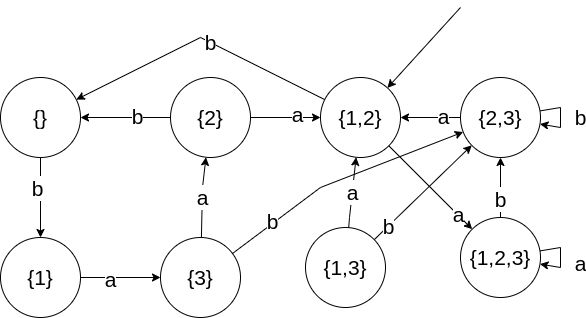
\includegraphics[scale=0.7]{02/HW02-1.16.b.png}    
\end{center}
\newpage
\section*{Problem 3}

Use the procedure described in Lemma 1.55 to convert the following regular ex-
pressions to nondeterministic finite automata. (page 86).
\newline
\newline
\textbf{1.19.a.} $(0\cup1)*000(0\cup1*)$

\begin{center}
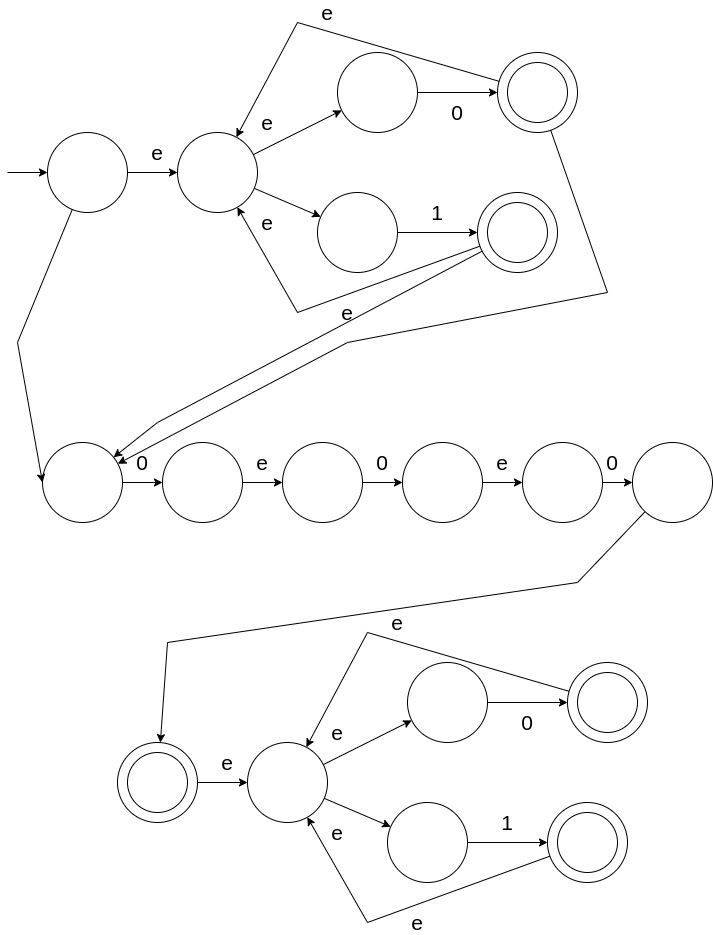
\includegraphics[scale=0.4]{02/HW02-1.19.a.png} 
\end{center}
\newpage
\textbf{1.19.b.} $(((00)*(11))\cup01)*$
\begin{center}
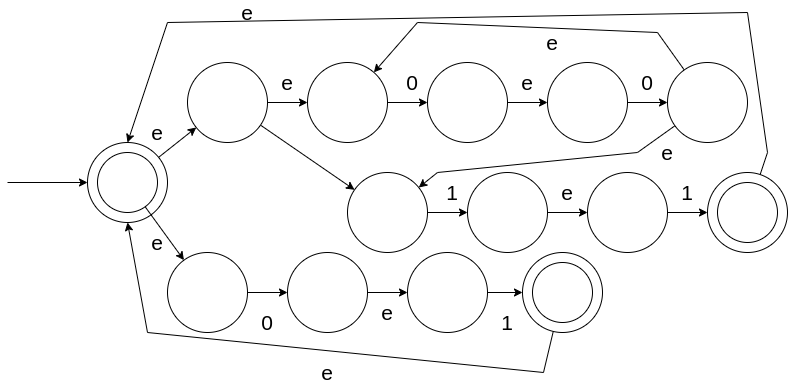
\includegraphics[scale=0.5]{02/HW02-1.19.b.png} 
\end{center}
\newpage
\section*{Problem 4}

Problem 1.21.a (page 86).
\begin{center}
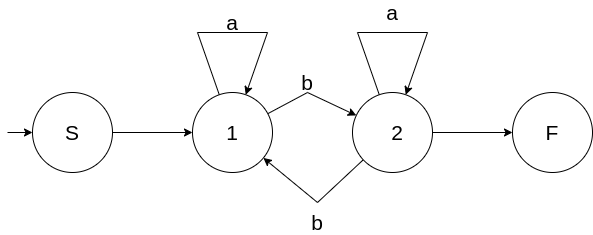
\includegraphics[scale=0.5]{02/HW02-1.21.a.png} 
\end{center}
\begin{center}
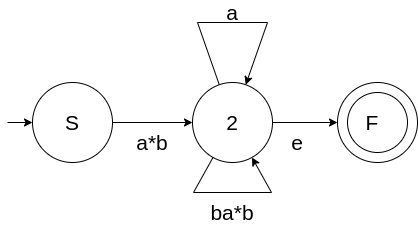
\includegraphics[scale=0.5]{02/HW02-1.21.b.png} 
\end{center}
\begin{center}
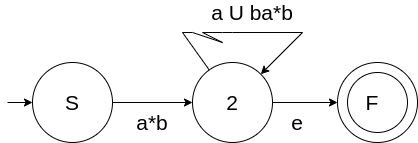
\includegraphics[scale=0.5]{02/HW02-1.21.c.png} 
\end{center}
\begin{center}
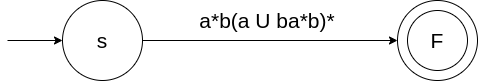
\includegraphics[scale=0.5]{02/HW02-1.21.d.png} 
\end{center}
The regular expression is: $a*b(a\cup ba*b)*$

\newpage
\section*{Problem 5}

Prove the following languages are not regular.
\newline
\newline
1. $xy^{i}z \in A$ for $i \geq 0$
\newline
2. $\mid y \mid > 0$
\newline
3. $\mid xy \mid \leq p$
%blem 1.23.a, 1.23.c (page 88).
\newline
\newline
\noindent
\textbf{(5.1)} $A=\{a^{n^3}|n\geq 0\}$. Here $a^x$ means a string of $x$ $a$'s.
\newline
\begin{proof}
Assume that $A$ is regular. Let $S = a^{p^{3}}$ where $p$ is the pumping length. By the pumping lemma, $S$ decomposes into $xyz$ s.t.
\newline
\newline
\noindent
By 3, $\mid y \mid \leq p$.
\newline
Pumping up, $\mid xy^{2}z \mid \leq p^{3} + p < p^{3} + 3p^{2} +3p +1 = (p+1)^{3}$.
\newline
By 2, $\mid y \mid > 0$, hence $p^{3} < \mid xy^{2}z \mid < (p+1)^{3}$. Thus $xy^{2}z \in A$, a contradiction of the pumping lemma.
\newline
\noindent
$\therefore$ $A$ is not regular.
\end{proof}

\noindent
\textbf{(5.2)} $B=\{0^n1^m0^n|m,n\geq 0\}$.
\newline
\begin{proof}
Assume $B$ is regular. Let $S = 0^{P}10^{P}$ where $p$ is the pumping length. Then, $S$ decomposes in $xyz$ s.t.
\newline
\newline
By 3, $y$ consists of only 0's.
\newline
Let $\delta = \mid y \mid$ then by 2, $\delta > 0$.
\newline
The pumping up, $xy^{2}z = 0^{P+\delta}10^{P} \notin B$ because the same number of 0's is not the same before and after the 1.
\newline
A contradiction of the pumping lemma.
\newline
$\therefore$ $B$ is not regular.
\end{proof}

\end{document}